\input{../../../utils/header_article.tex}

\usepackage{graphicx}
\newcommand\sbullet[1][.5]{\mathbin{\vcenter{\hbox{\scalebox{#1}{$\bullet$}}}}}
\usepackage[export]{adjustbox}

\title{Causal Graphs\thanks{We are indebted to Liudmila Kiseleva for the design of the handout.}}
\subtitle{Definitions, patterns, and strategies}
\date{}

\begin{document}\maketitle\vspace{-2cm}

\section*{Definitions}

\begin{itemize}

\item A \textbf{node} represents a random variable labeled by letter. Observed random variables are marked by solid circle $\bullet$ and unobserved - by hollow circle \( \circ \).

\item An \textbf{edge} shows dependence between joining variables.

\item \textbf{Adjacent variables} are connected by an edge.

\item \textbf{Adjacent edges} meet at a variable.

\item A \textbf{directed edge} represents the cause by a single-headed arrow.

\item A \textbf{parent/child} is the starting(tail)/ending(head) variable. Therefore, a directed edge represents a direct effect of a parent on a child.

\item A \textbf{root} is a variable that has no parent. In other words, it is an exogenous variable determined only by forces outside of the graph.

\item A \textbf{sink} is a variable with no children.

\item A \textbf{path} is a sequence of adjacent edges.

\item A \textbf{directed path} is a path traced out entirely along arrows tail-to-head. If there is a directed path from A to B,  A is an \textbf{ancestor} of B; B is a  \textbf{descendant} of A.

\item A \textbf{directed acyclic graph (DAG)} is a graph with only arrows for edges and no feedback loops (i.e. no variable is its own ancestor or its own descendant):

\begin{figure}[htp]\centering
\caption{Directed acyclical graph}
\scalebox{0.05}{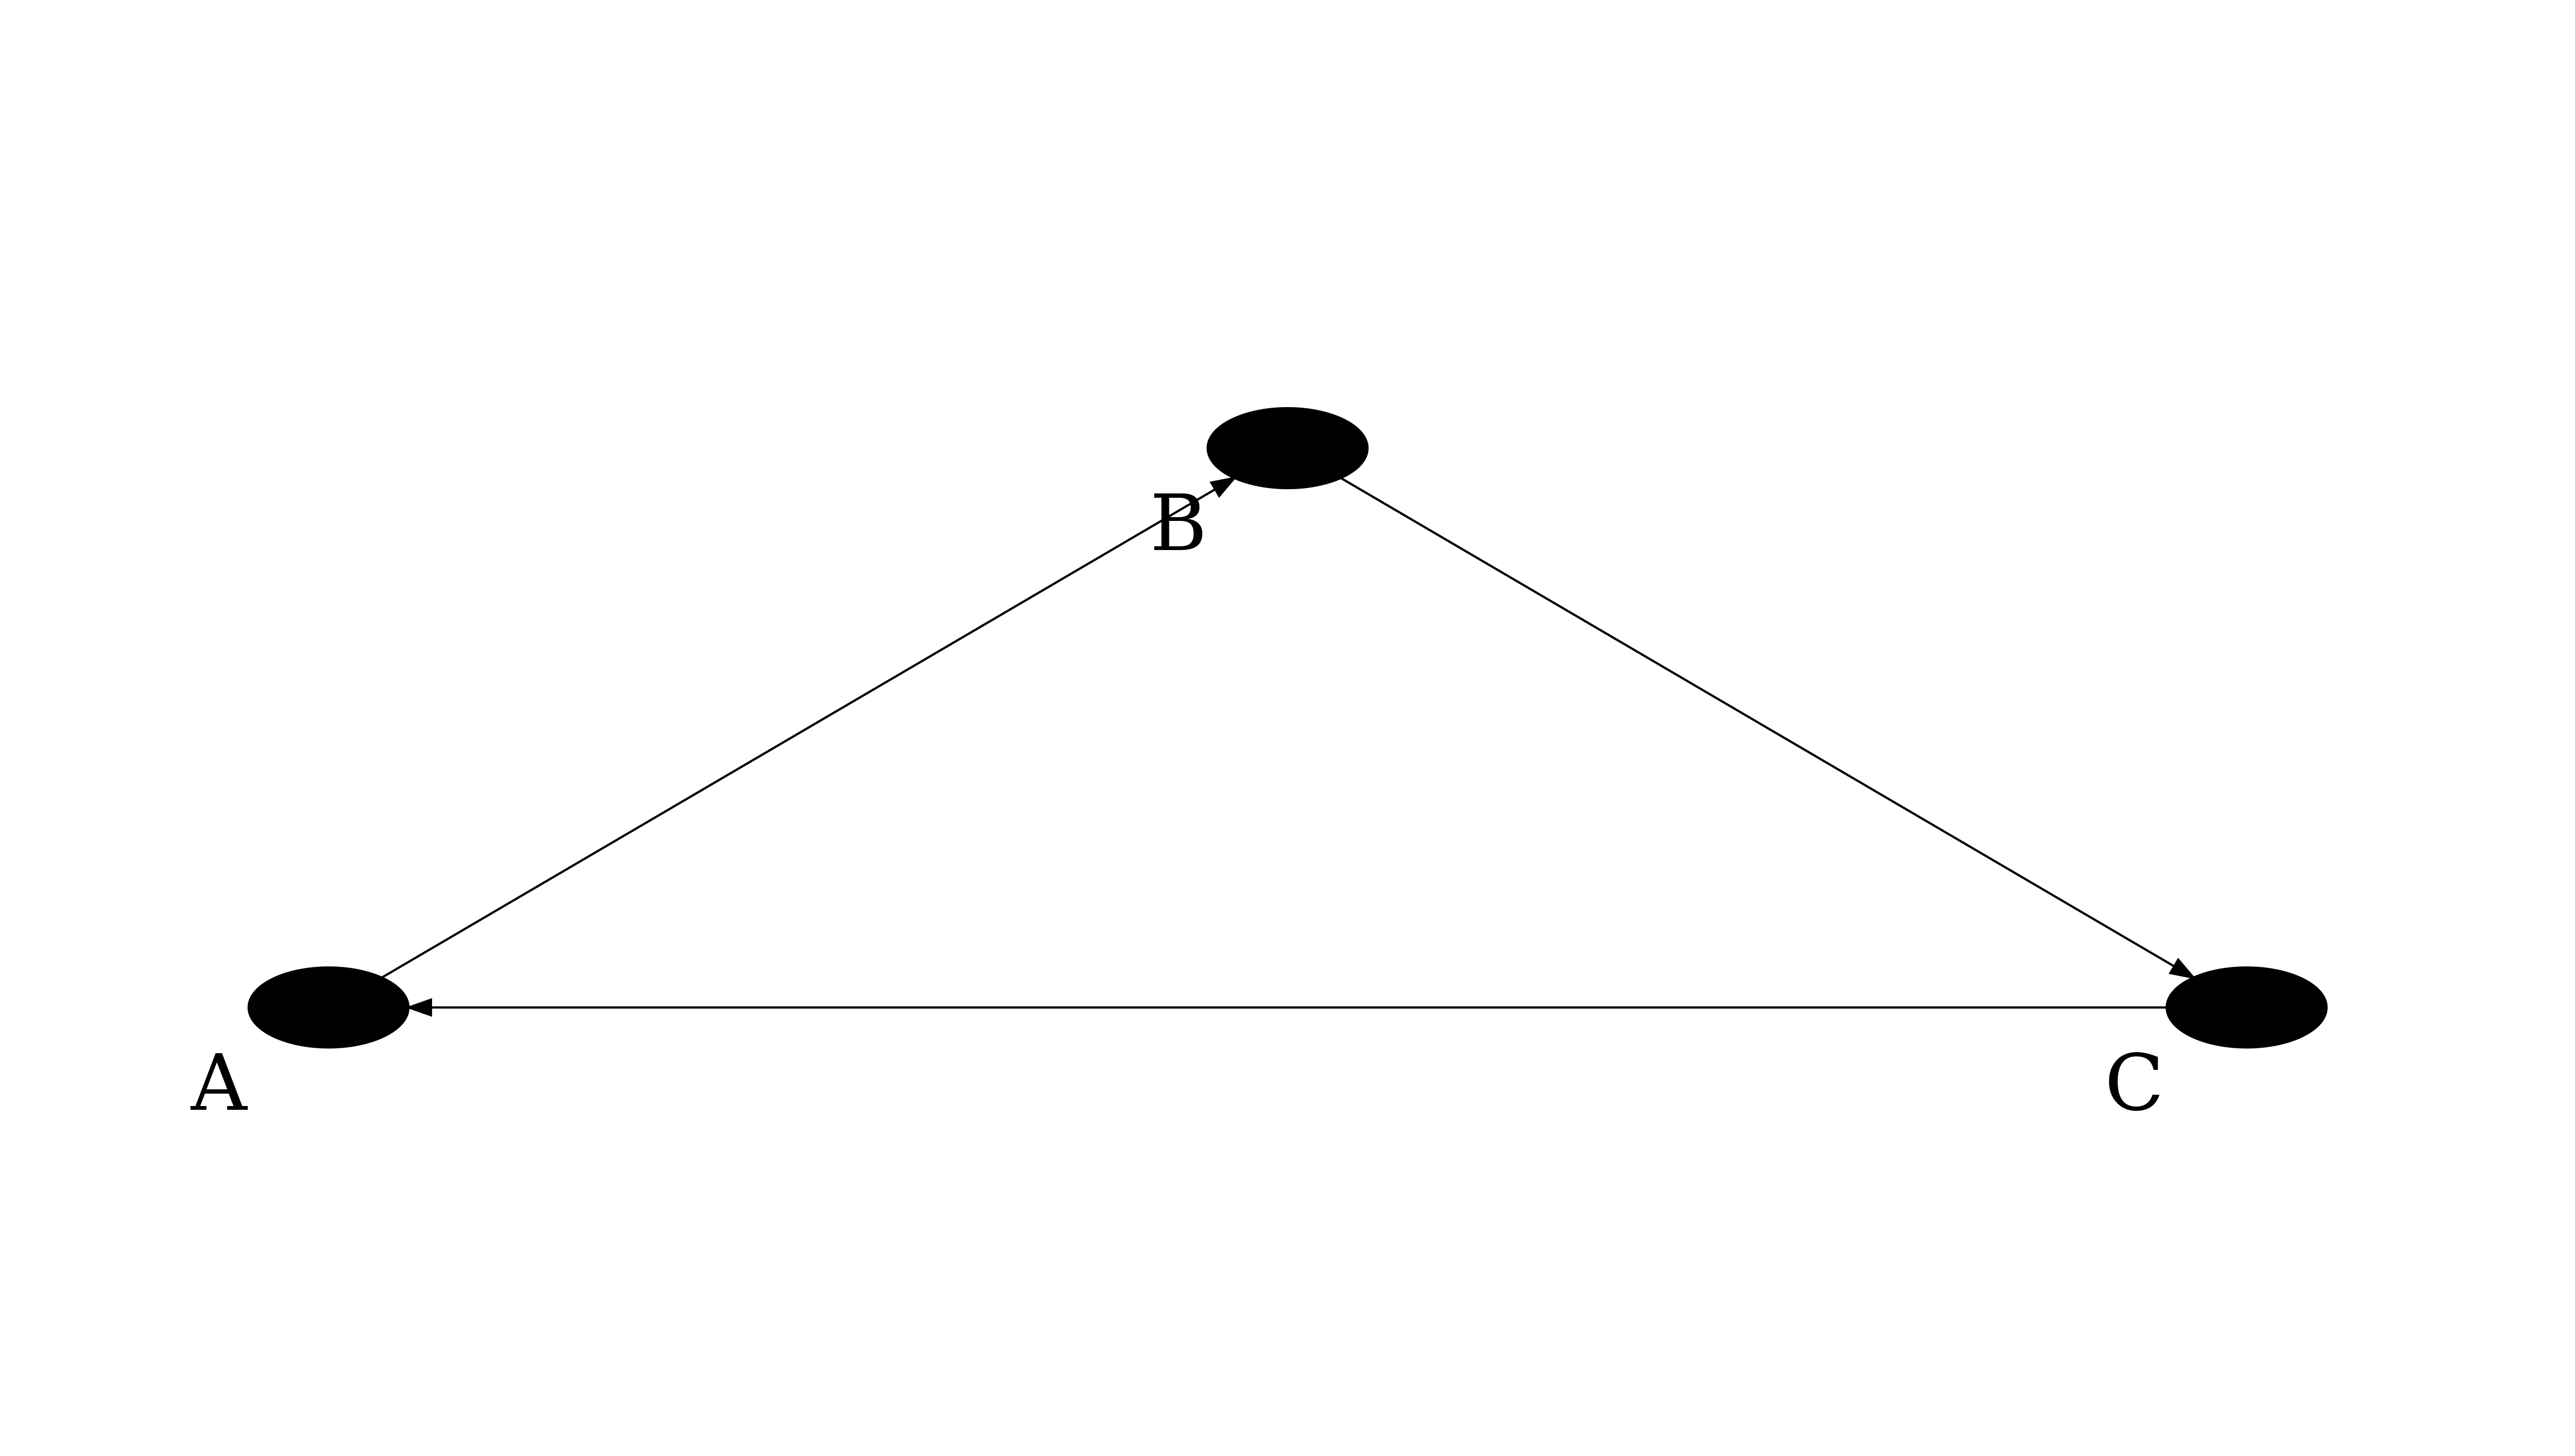
\includegraphics{../materials/fig-1-handout}}
\end{figure}

\item \textbf{Mutual dependence} of two variables on one or more common causes is shown:

\begin{figure}[htp]\centering
\caption{Mutual dependence}\
\scalebox{0.05}{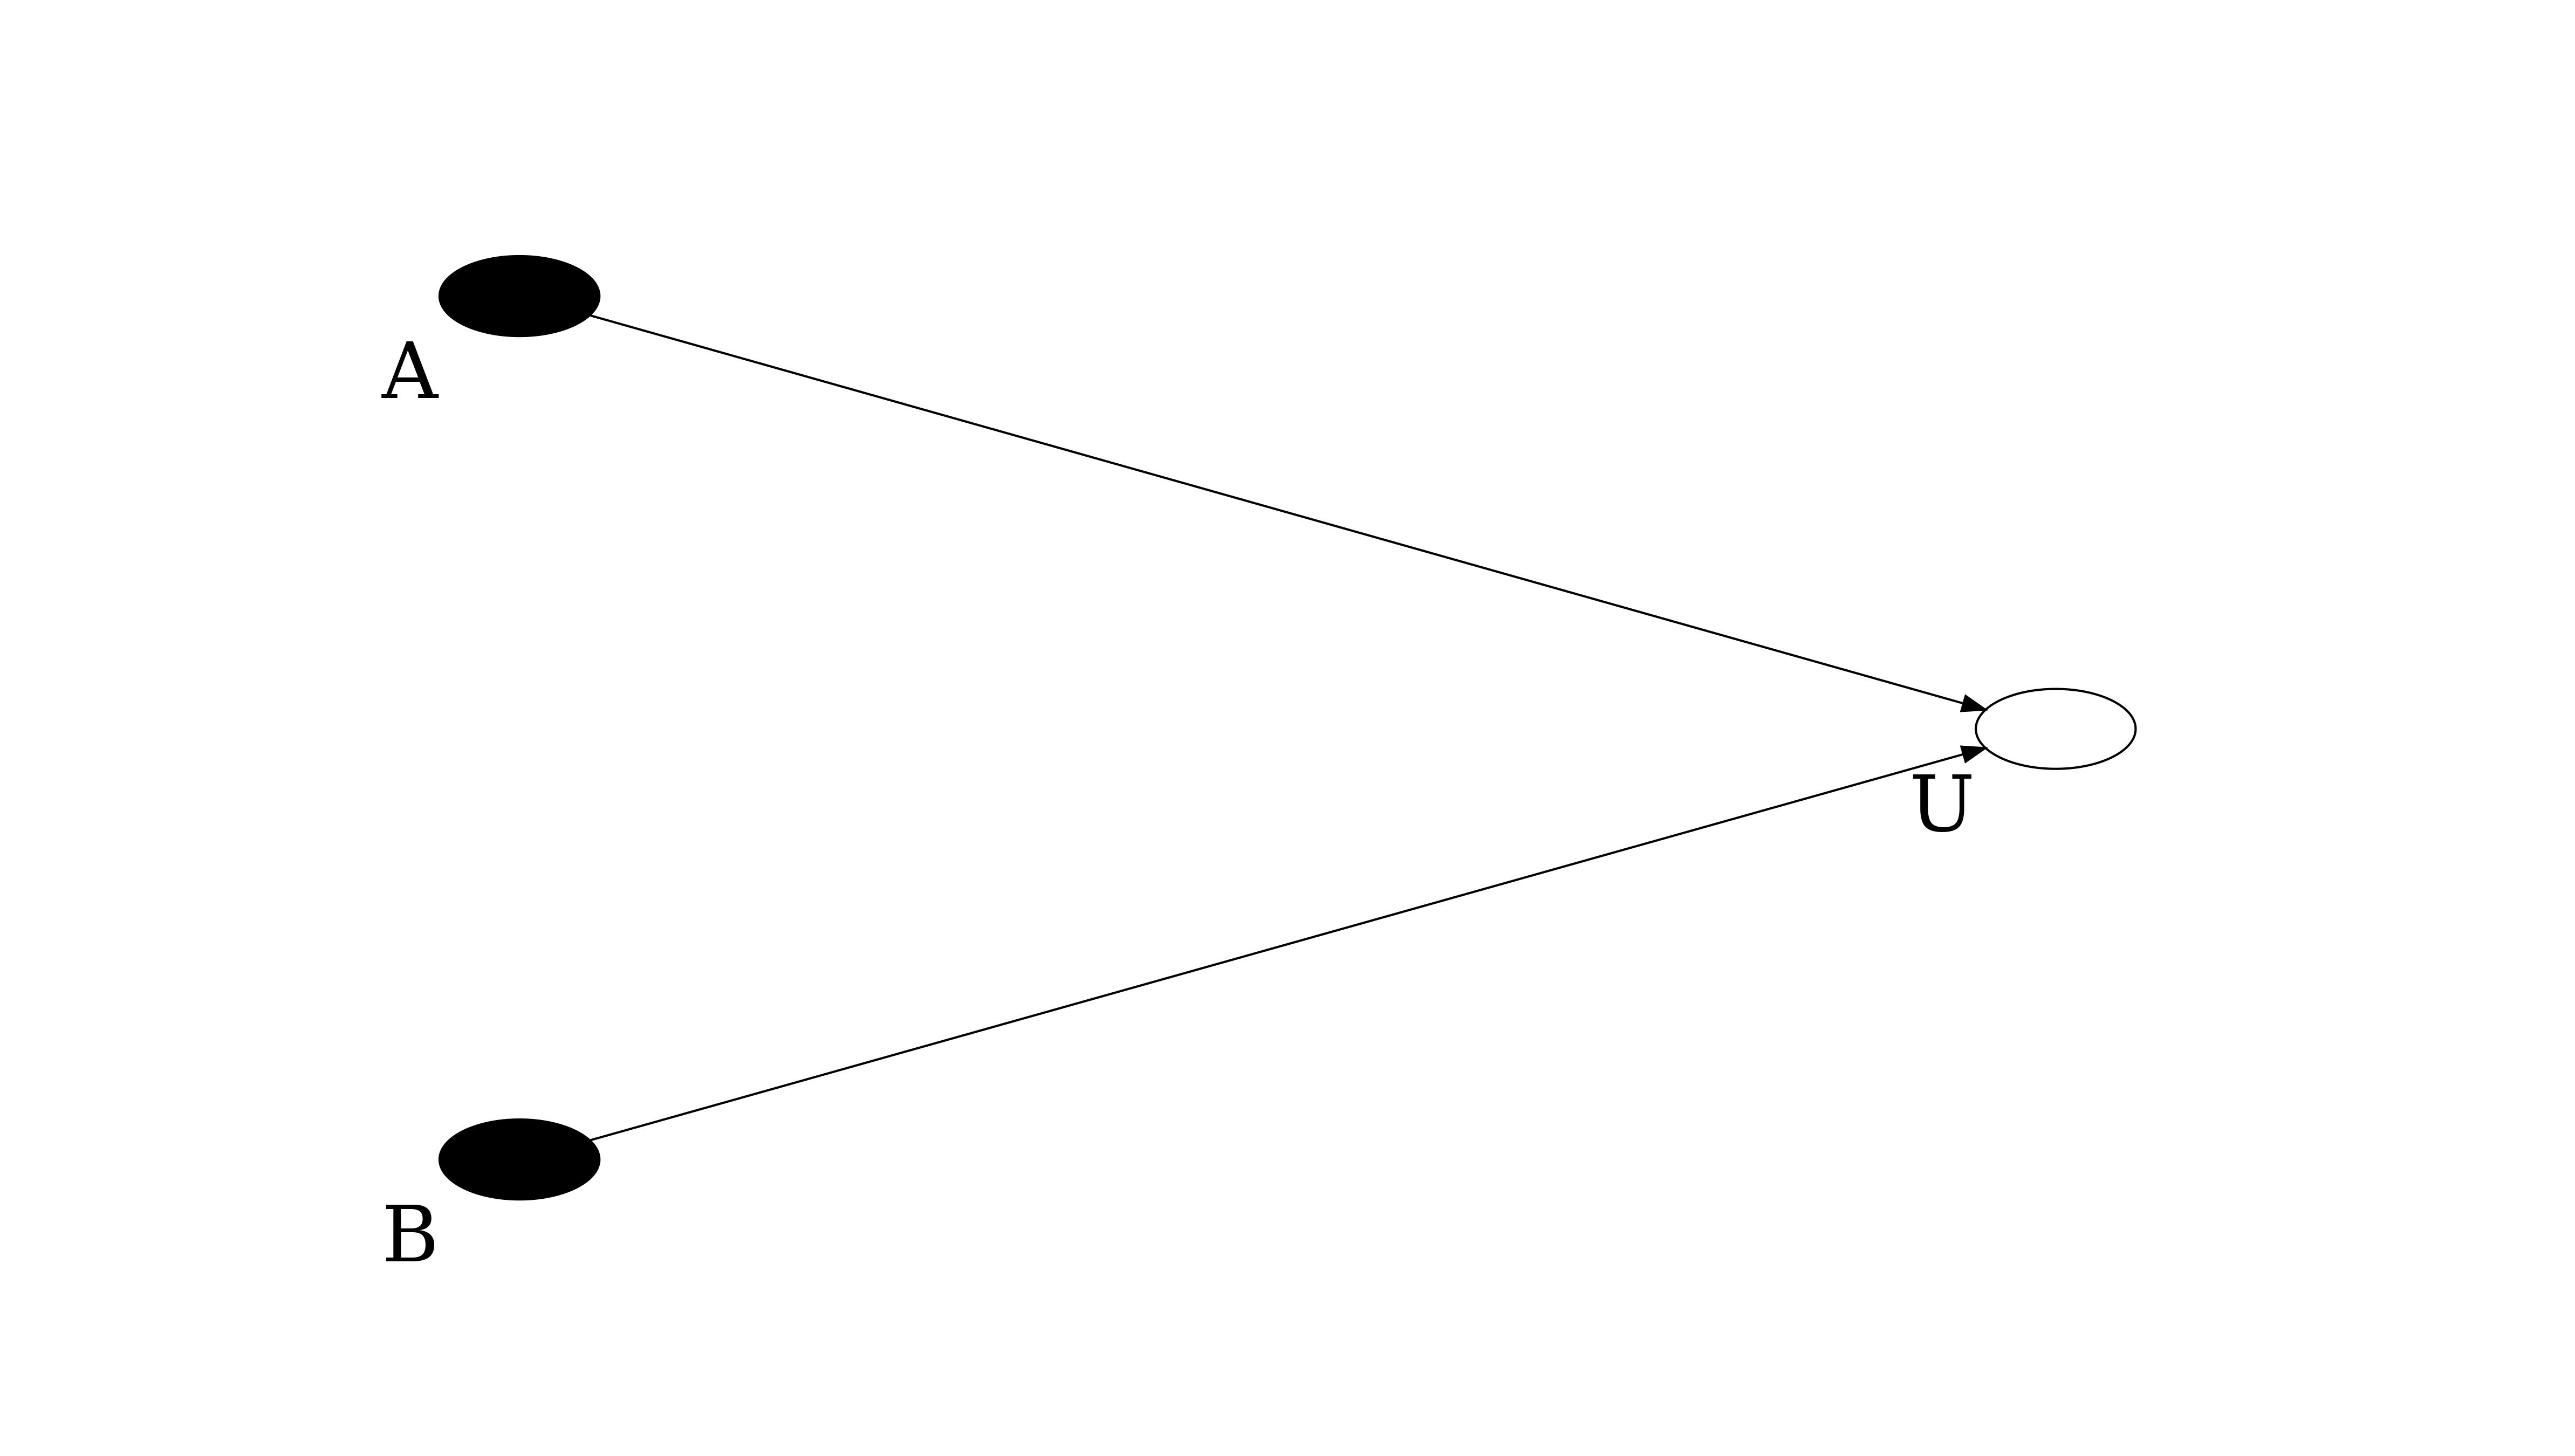
\includegraphics{../materials/fig-2-b-handout}}
\end{figure}

\end{itemize}

\section*{Patterns}

\begin{itemize}

\item \textbf{Chain of mediation} is a relationship when A affects B through A's causal effect on C and C's causal effect on B.

\begin{figure}[htp]\centering
\caption{Mediation}\
\scalebox{0.05}{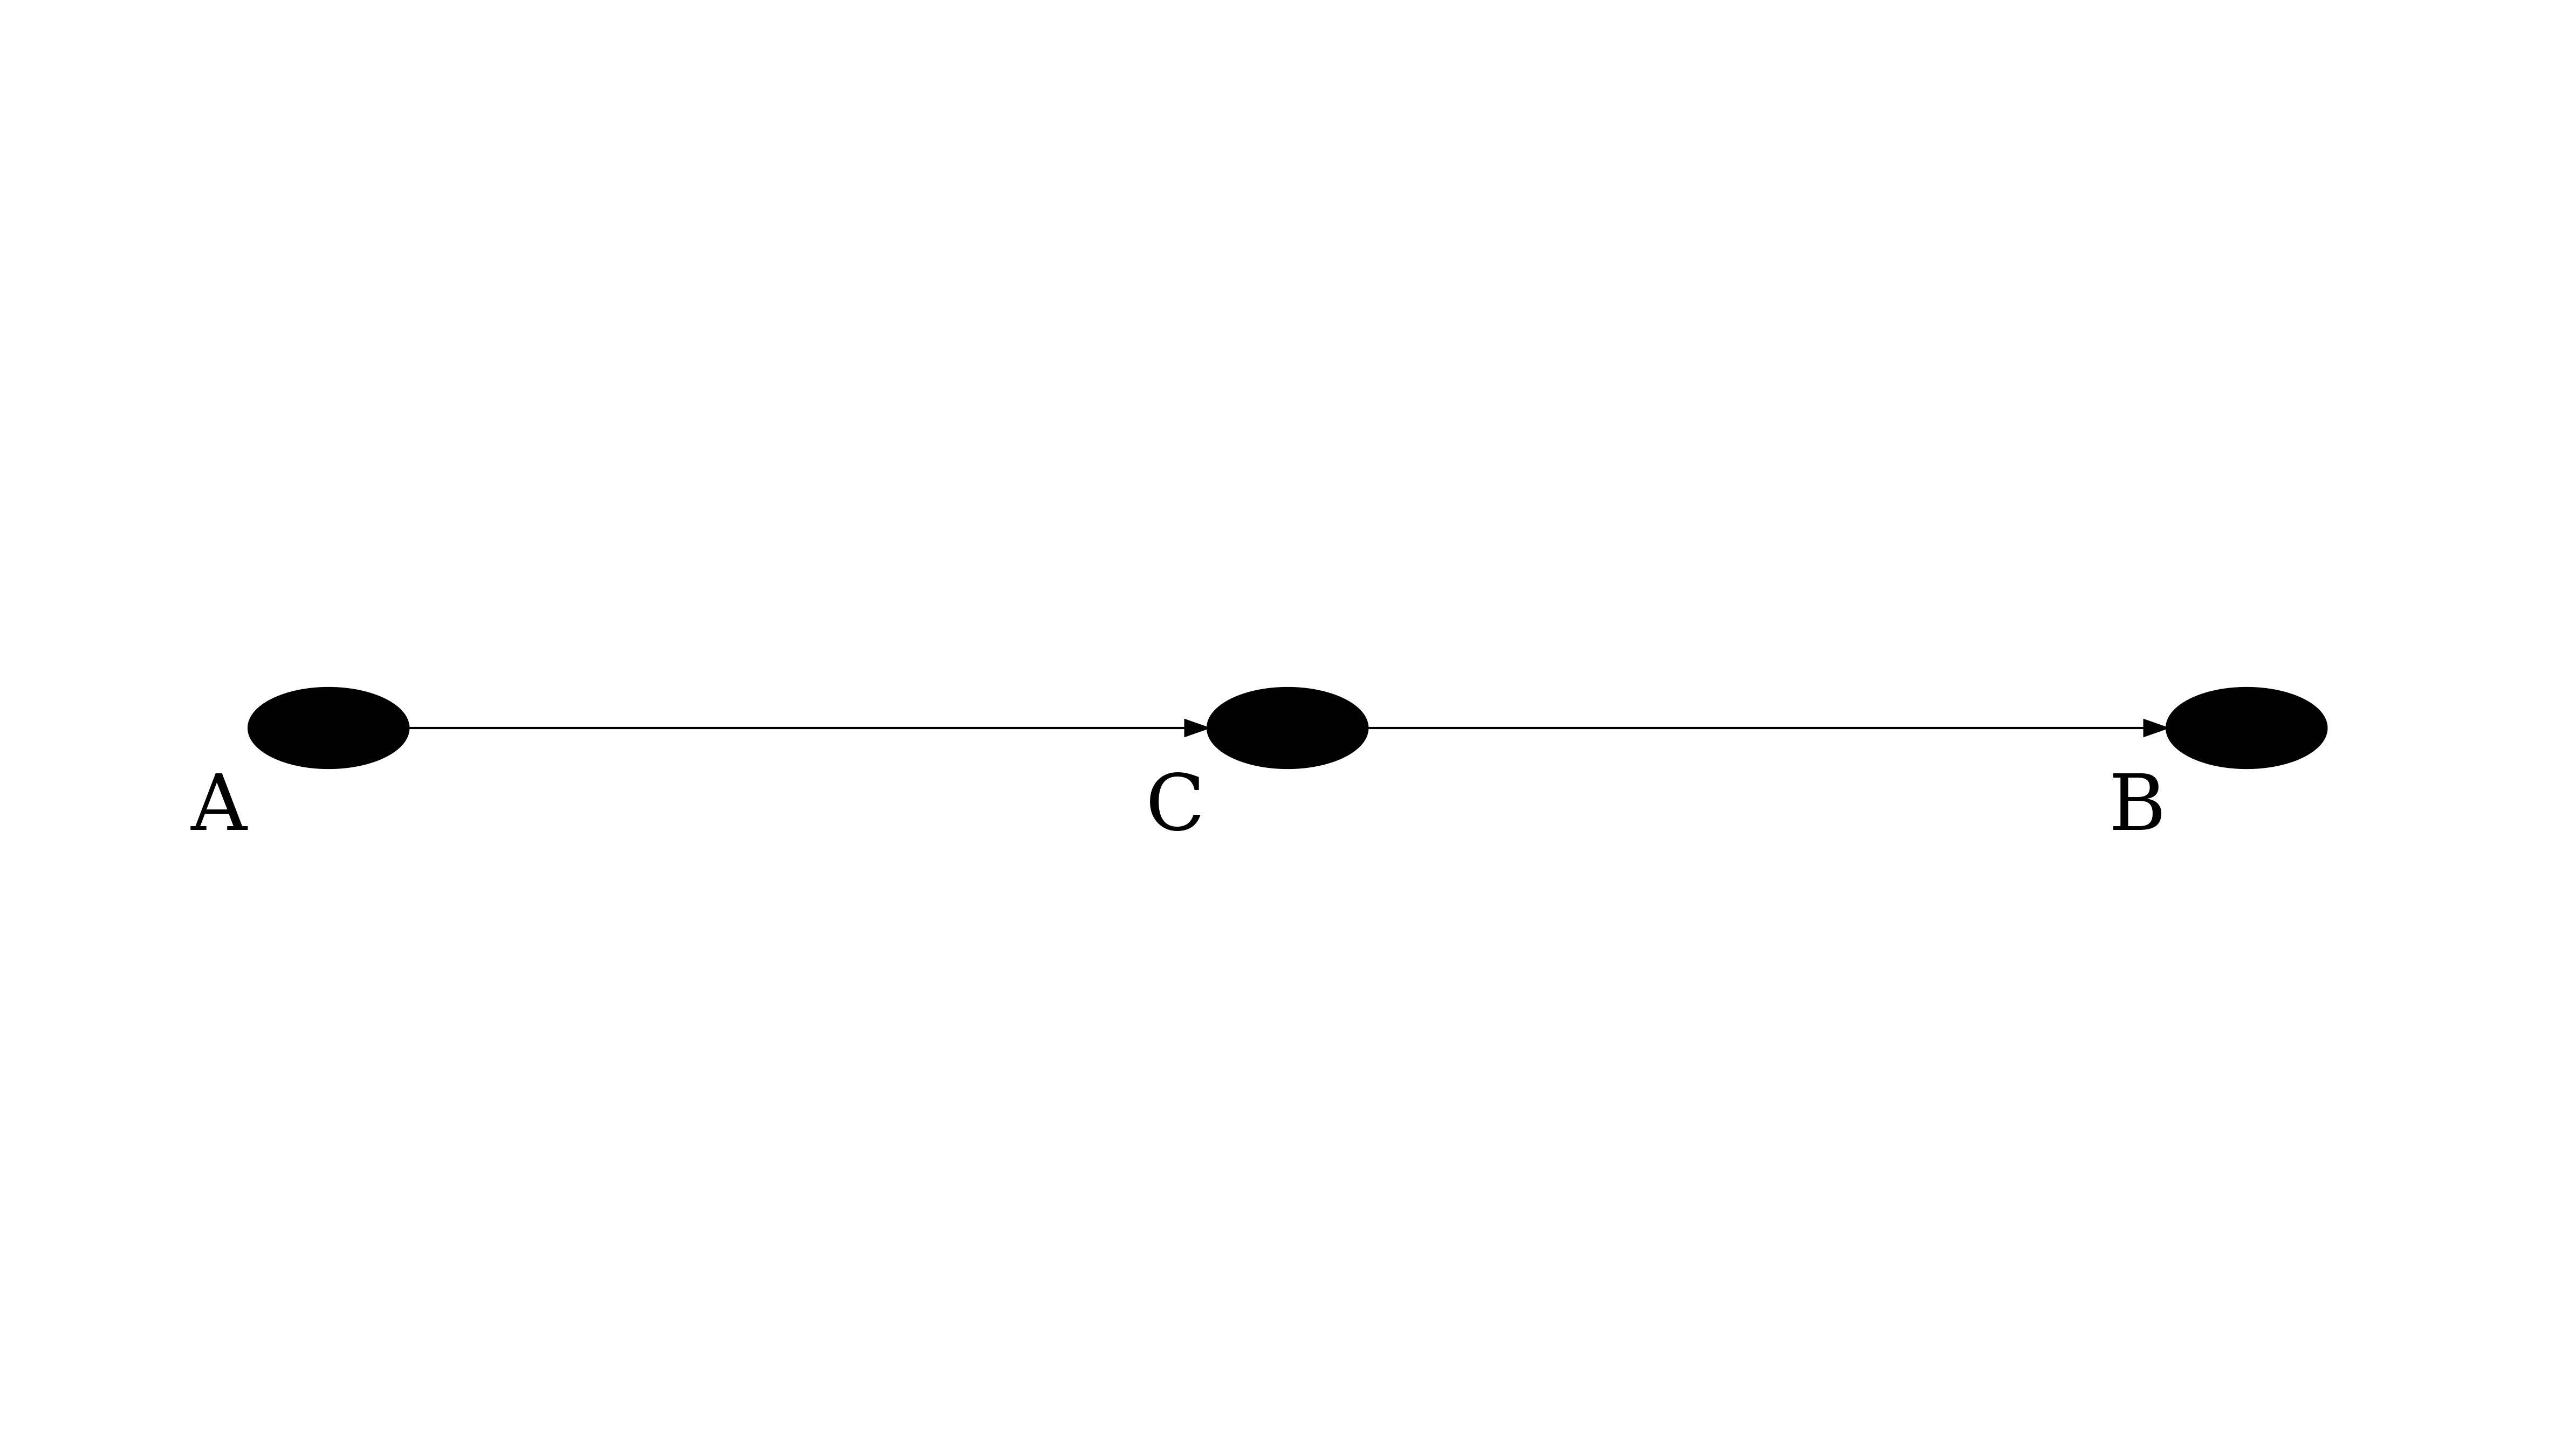
\includegraphics{../materials/fig-3-handout}}
\end{figure}

\item \textbf{Mutual dependence} is a relationship when A and B are both caused by C.

\item A \textbf{confounding variable} is a variable that affects both the dependent and independent variable.

\begin{figure}[htp]\centering
\caption{Mutual dependence}\
\scalebox{0.05}{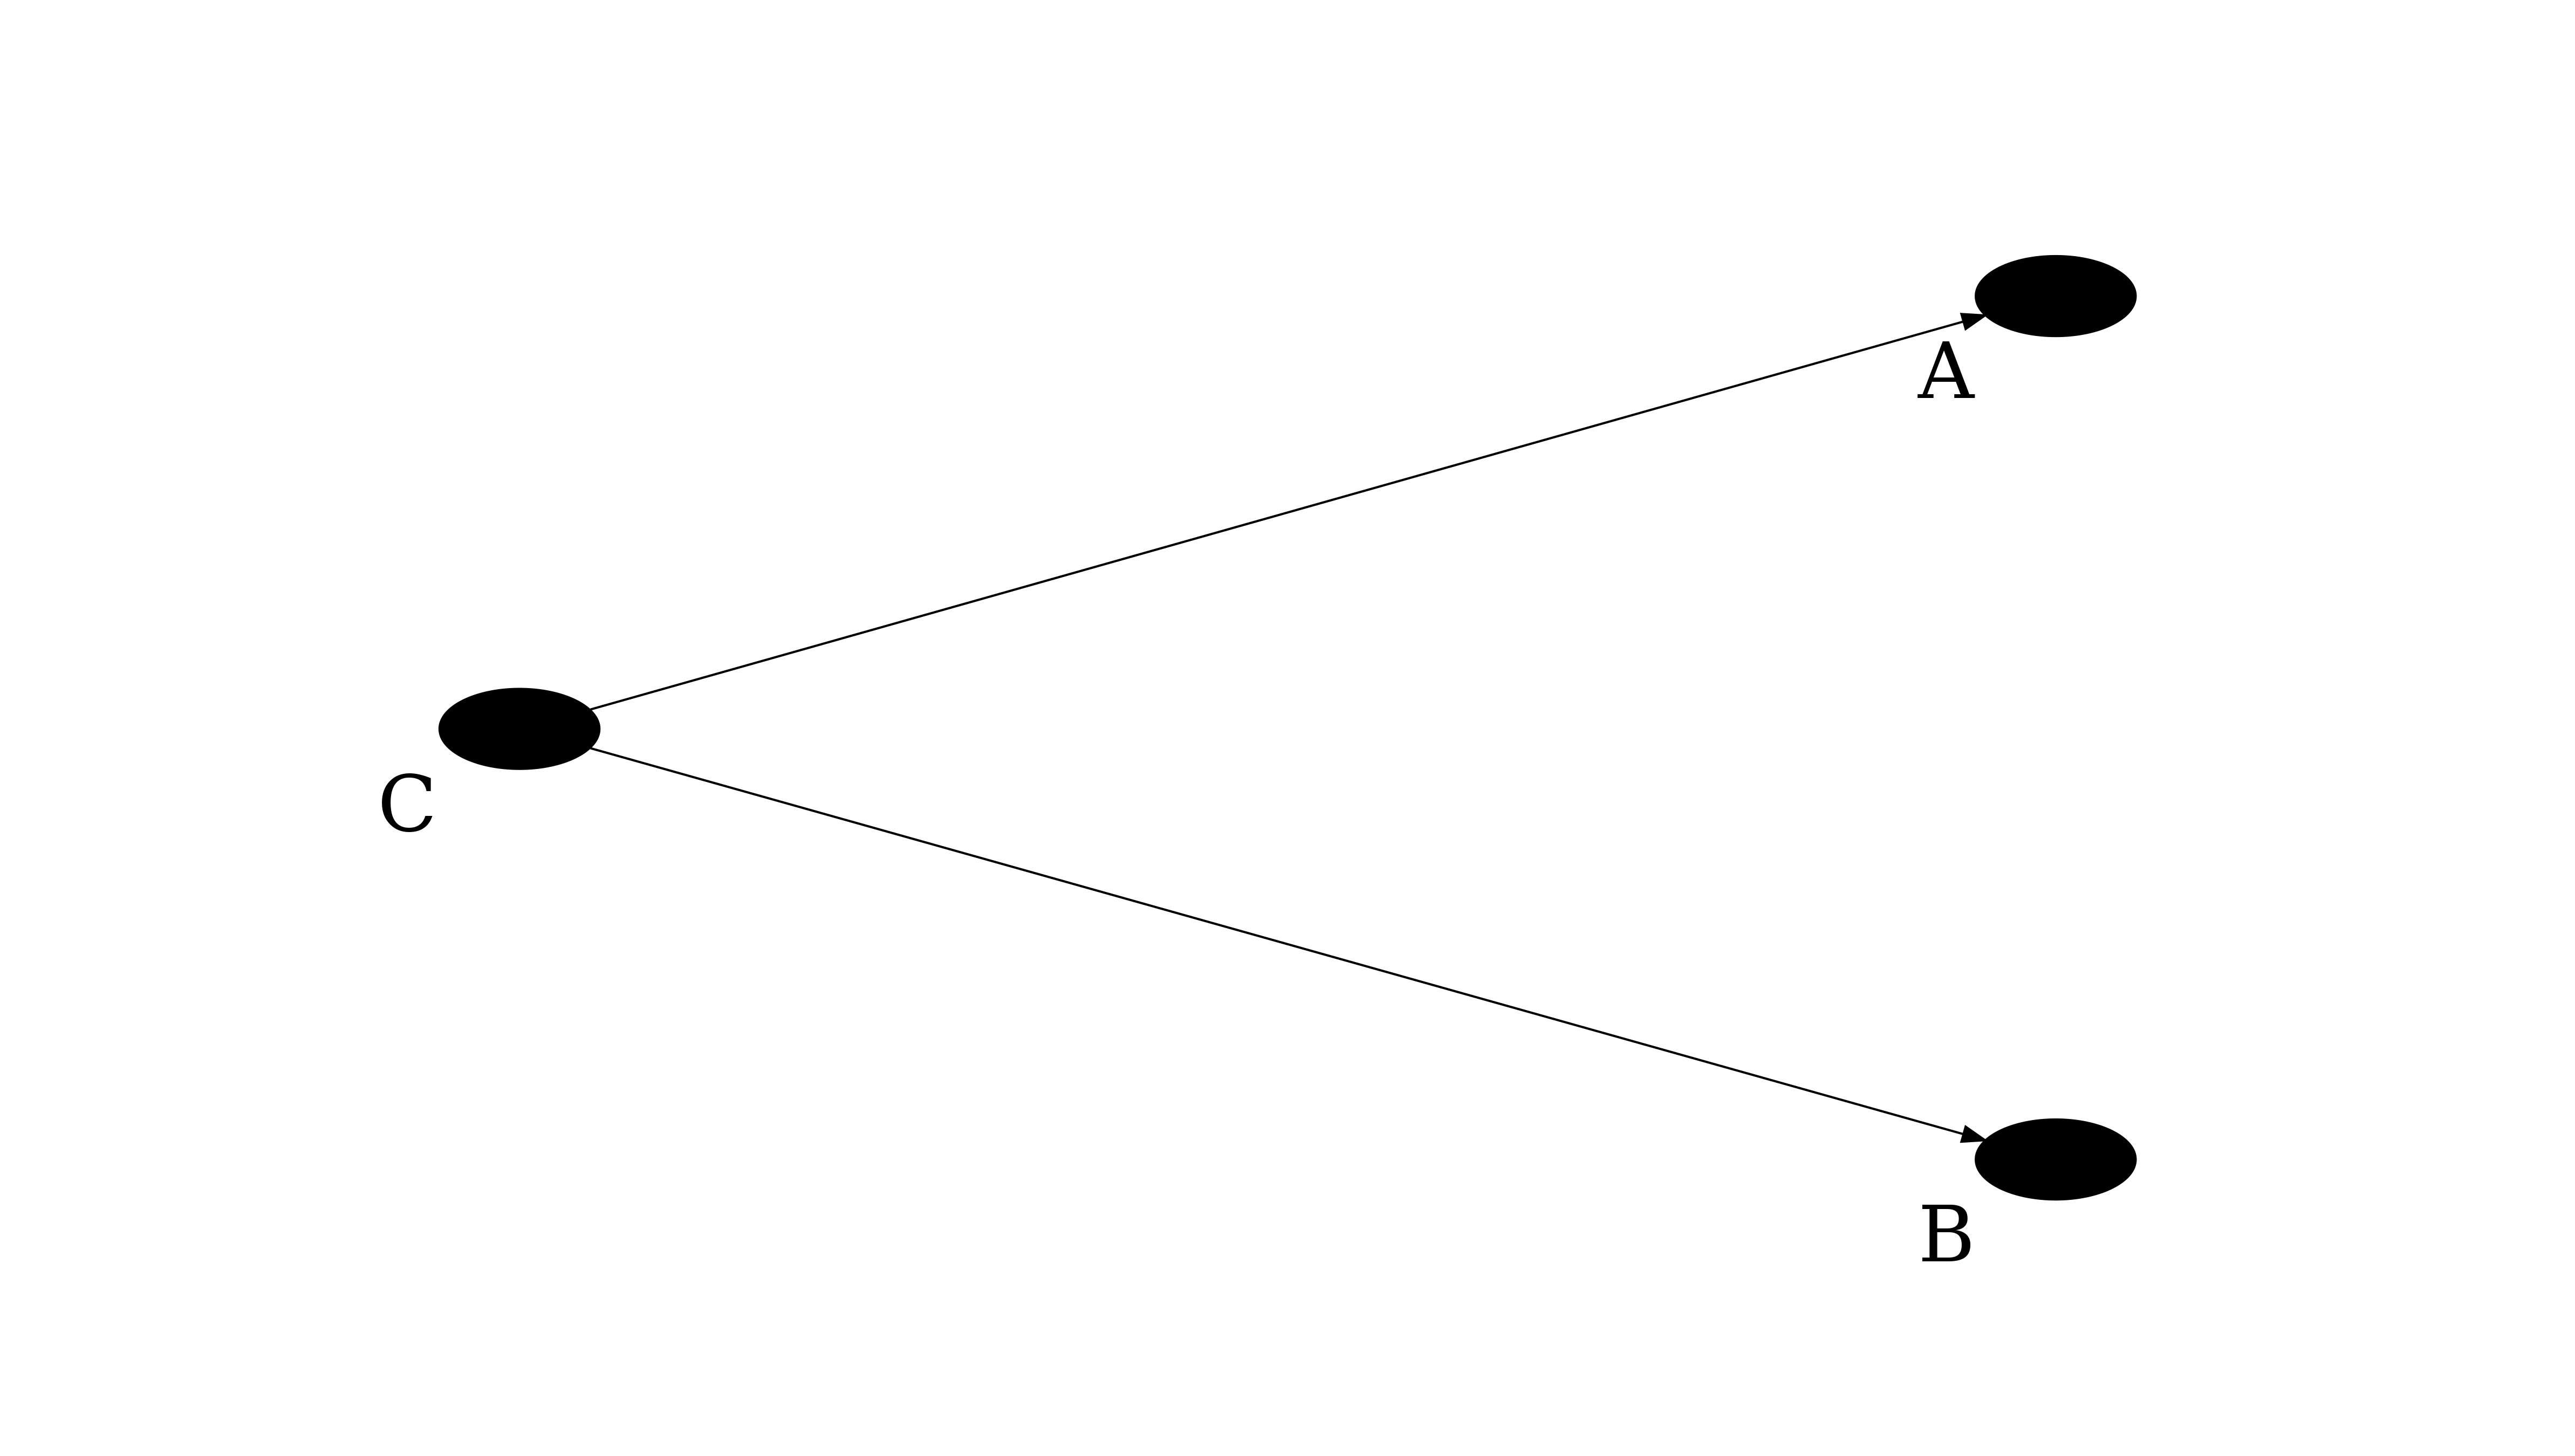
\includegraphics{../materials/fig-4-handout}}
\end{figure}

\item \textbf{Mutual causation} is a relationship when A and B are both causes of C. 

\item A \textbf{collider} is a variable that has two arrows running into it.

\begin{figure}[htp]\centering
\caption{Mutual causation}\
\scalebox{0.05}{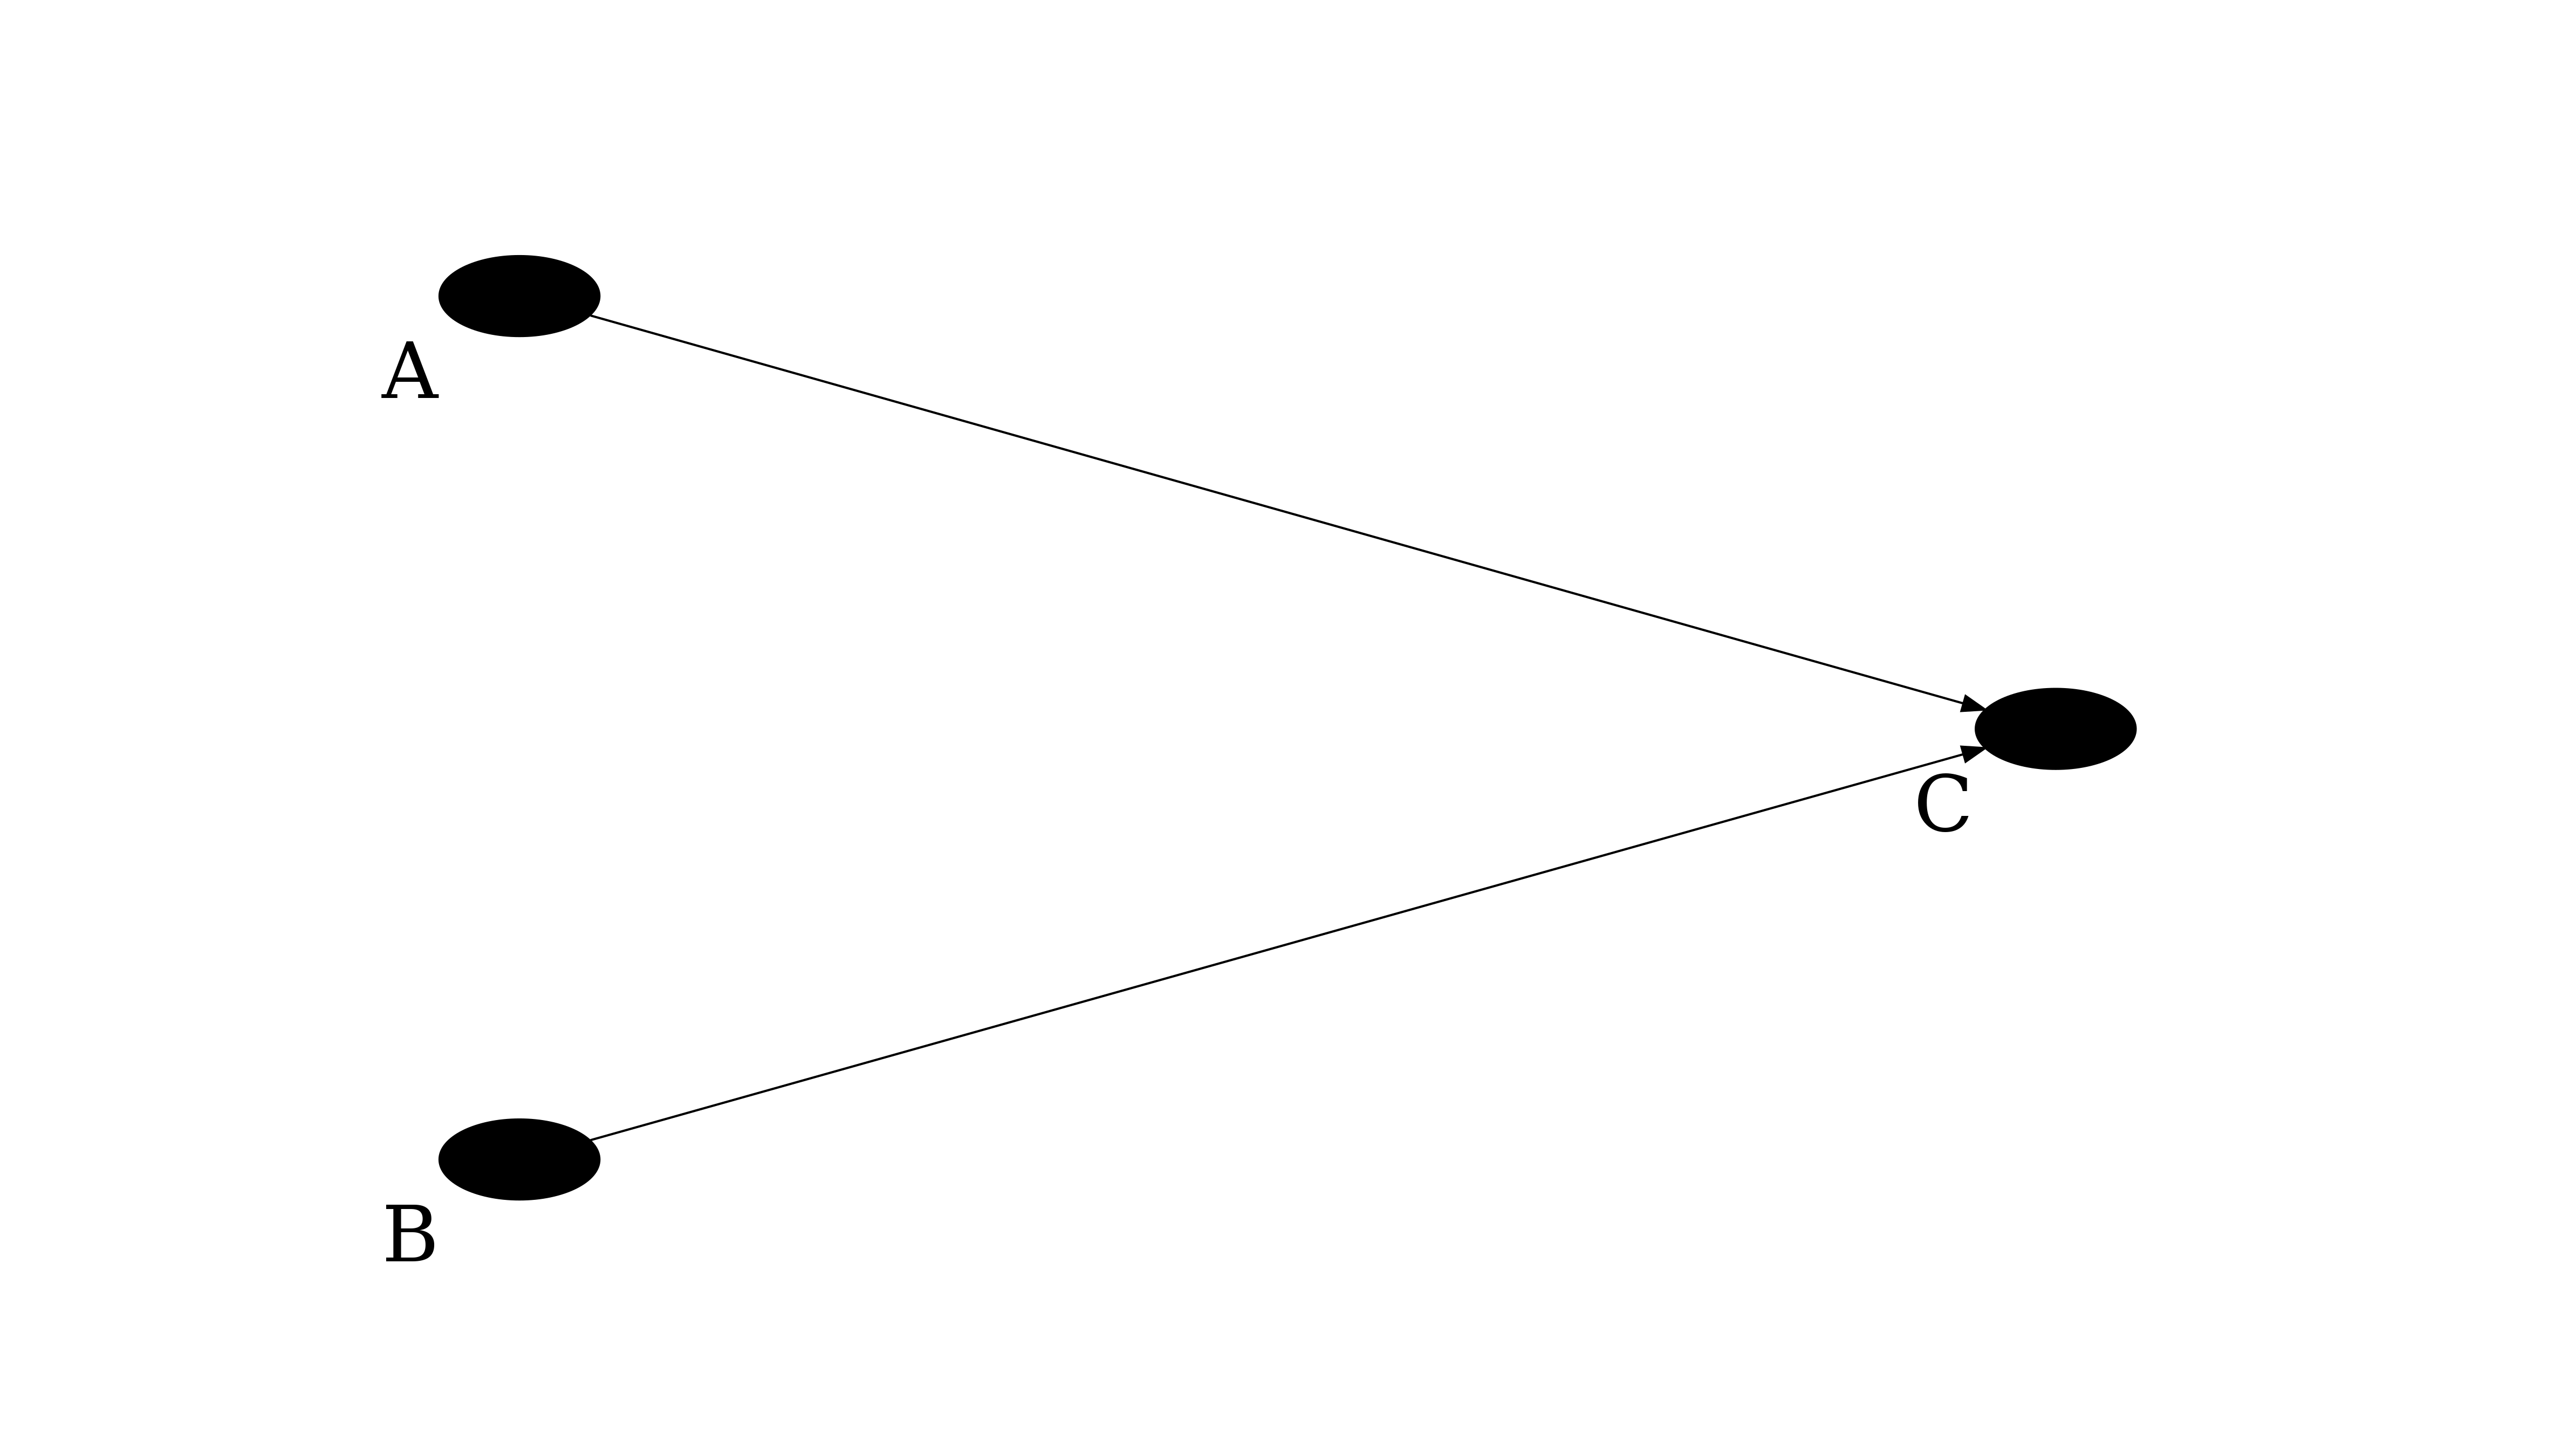
\includegraphics{../materials/fig-5-handout}}
\end{figure}

\item A \textbf{back-door path} is a path between any causally ordered sequence  of two variables that include a directed edge that points to the first variable. 

\item \textbf{Conditioning} as a modeling strategy means transforming one graph into a simpler set of component graphs where fewer causes are represented.

\end{itemize}

\section*{Strategies}

A \textbf{back-door criterion} is a set of conditions used to determine whether or not conditioning on a given set of observed variable will identify the causal effect. The causal effect is identified by conditioning on a set of variables Z if and only if all back-door paths between the causal variable and the outcome variable are blocked after conditioning on Z. All back-door paths are blocked by Z if and only if each back-door path:

\begin{itemize}

\item contains a chain of mediation A $\rightarrow$ C $\rightarrow$  B where the middle variable C is in Z, or

\item contains a fork of mutual dependence A $\leftarrow$ C $\rightarrow$ B, where the middle variable C is in Z, or

\item contains an inverted fork of mutual causation A $\rightarrow$ C $\leftarrow$  B, where the middle variable C and all of C's decendents are not in Z.

\end{itemize}

A \textbf{front-door criterion} is an empirical strategy used to identify the causal relationship flowing from A to B if one can find a mechanism C which:

\begin{itemize}

\item  lies on the causal path between A and B, and 

\item it is the only such mechanism, and 

\item it is not affected by the unobserved confounder U.

\end{itemize}

\begin{figure}[htp]\centering
\caption{Front-door criterion}\
\scalebox{0.05}{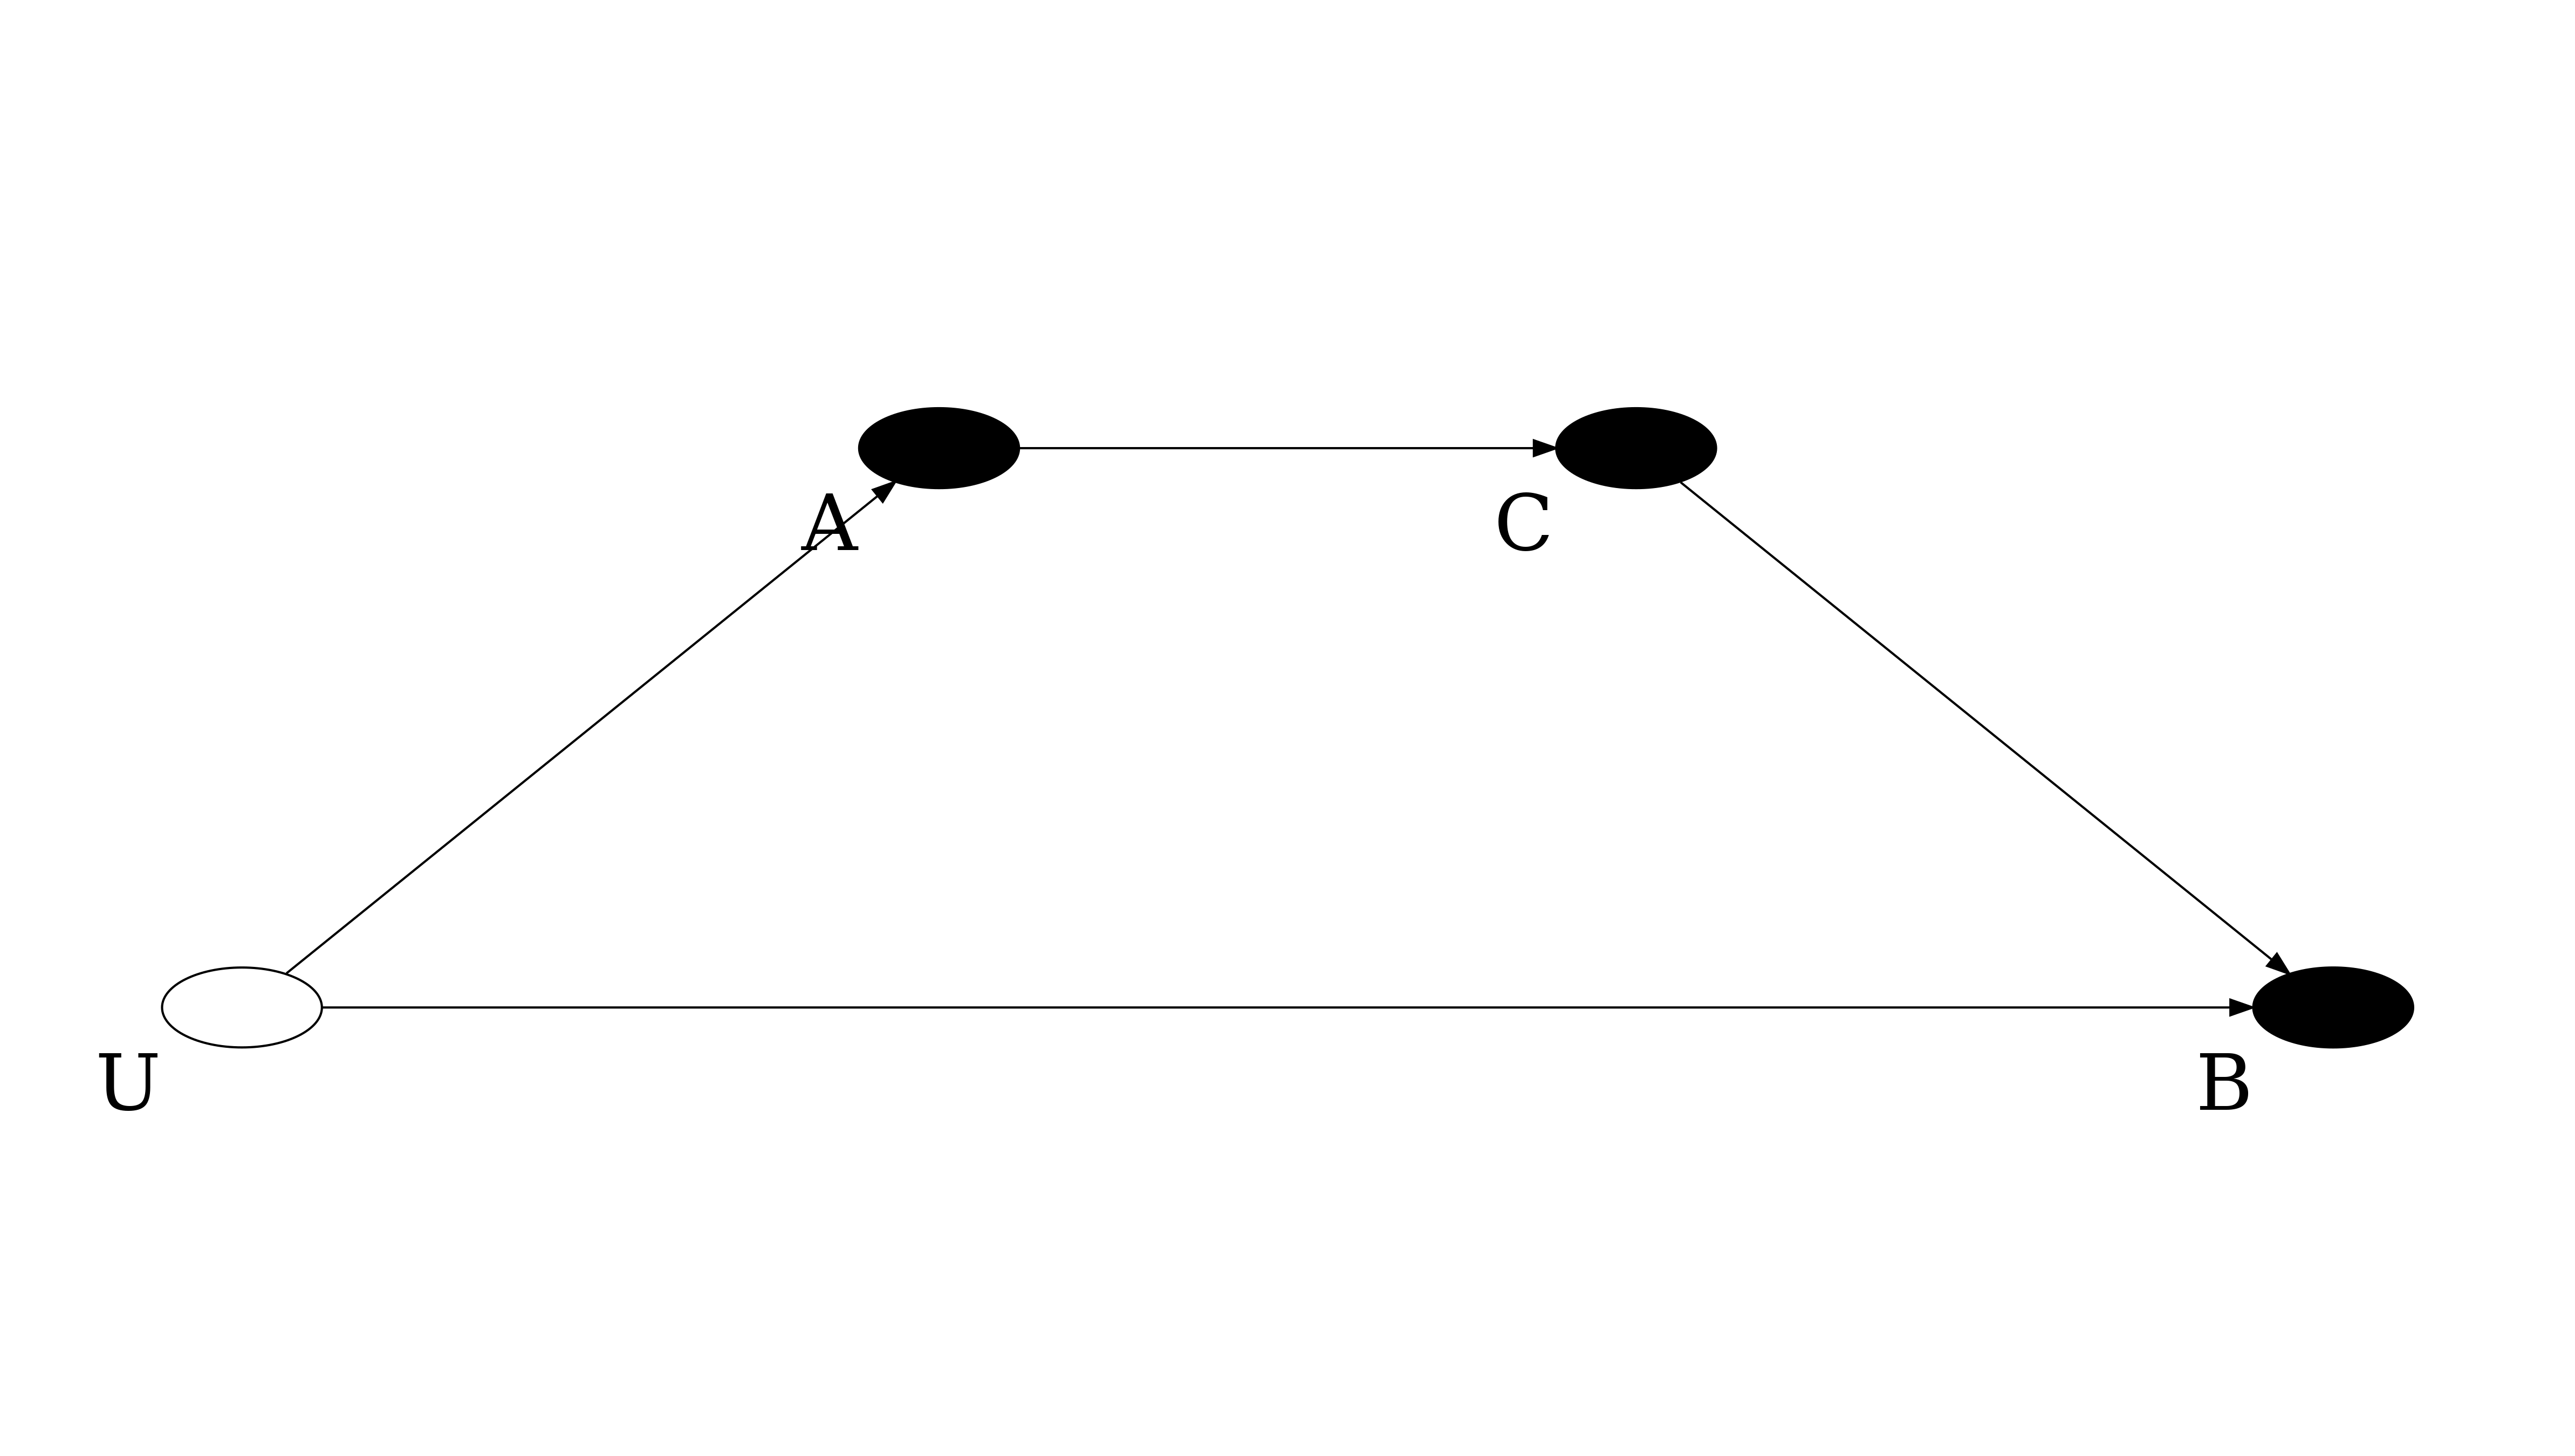
\includegraphics{../materials/fig-6-handout}}
\end{figure}

You can find more on front-door criterion application in the \cite{Bellemare.2020} paper.

\nocite{Morgan.2014}
\nocite{Pearl.2009}

\bibliographystyle{apacite}
\bibliography{../../../submodules/bibliography/literature}

\end{document}
